\section{Risposte alle domande}

\subsection{Domanda 1}

\textit{Eseguite i tre algoritmi che avete implementato (Held-Karp, euristica costruttiva e 2-approssimato) sui 13 grafi
del dataset. Mostrate i risultati che avete ottenuto in una tabella come quella sottostante. Le righe della tabella
corrispondono alle istanze del problema. Le colonne mostrano, per ogni algoritmo, il peso della soluzione trovata, il
tempo di esecuzione e l'errore relativo calcolato come $(SoluzioneTrovata - SoluzioneOttima) / SoluzioneOttima$. Potete
aggiungere altra informazione alla tabella che ritenete interessanti.}

Abbiamo implementato il codice in Python per l'esecuzione dei tre algoritmi su tutto il dataset fornito. Nella tabella che segue sono riportate le soluzioni ottime dei diversi dataset come riferimento per i risultati che abbiamo ottenuto.

\begin{table}[H]
  \centering
  \begin{tabular}{|l|c|c|c|}
  \hline
  \multicolumn{1}{|c|}{\textbf{File}} & \textbf{Descrizione} & \textbf{N} & \textbf{Soluzione Ottima} \\ \hline
  \textit{berlin52.tsp} & Berlino & 52 & 7542 \\ 
  \textit{burma14.tsp} & Birmania (Myanmar) & 14 & 3323 \\ 
  \textit{ch150.tsp} & Random & 150 & 6528 \\ 
  \textit{d493.tsp} & Foratura di circuiti stampati & 493 & 35002 \\ 
  \textit{dsj1000.tsp} & Random & 1000 & 18659688 \\ 
  \textit{eil51.tsp} & Sintetico & 51 & 426 \\ 
  \textit{gr202.tsp} & Europa & 202 & 40160 \\ 
  \textit{gr229.tsp} & Asia/Australia & 229 & 134602 \\ 
  \textit{kroA100.tsp} & Random & 100 & 21282 \\ 
  \textit{kroD100.tsp} & Random & 100 & 21294 \\ 
  \textit{pcb442.tsp} & Foratura di circuiti stampati & 442 & 50778 \\ 
  \textit{ulysses16.tsp} & Mediterraneo & 16 & 6859 \\ 
  \textit{ulysses22.tsp} & Mediterraneo & 22 & 7013 \\ \hline
  \end{tabular}
  \caption{Soluzioni ottime per ogni algoritmo su ogni dataset.}
  \label{tab:opt-results}
  \end{table}

\subsubsection{Risultati e tempistiche}

I risultati sperimentali degli algoritmi da noi implementati sono riportati nella tabella alla pagina che segue.

\begin{landscape}
  %\thispagestyle{empty}
  % Please add the following required packages to your document preamble:
% \usepackage{multirow}
% Please add the following required packages to your document preamble:
% \usepackage{multirow}
\begin{table}[]
  \centering
  \begin{tabular}{|l|l|l|l|l|l|l|l|l|l|}
  \hline
  \multicolumn{1}{|c|}{\multirow{2}{*}{\textbf{Istanza}}} & \multicolumn{3}{c|}{\textbf{Held-Karp}} & \multicolumn{3}{c|}{\textbf{Nearest Neighbor}} & \multicolumn{3}{c|}{\textbf{2-approximation}} \\ \cline{2-10} 
  \multicolumn{1}{|c|}{} & \multicolumn{1}{c|}{\textbf{Soluzione}} & \multicolumn{1}{c|}{\textbf{\begin{tabular}[c]{@{}c@{}}Tempo\\ {[}s{]}\end{tabular}}} & \multicolumn{1}{c|}{\textbf{\begin{tabular}[c]{@{}c@{}}Errore\\ {[}\%{]}\end{tabular}}} & \multicolumn{1}{c|}{\textbf{Soluzione}} & \multicolumn{1}{c|}{\textbf{\begin{tabular}[c]{@{}c@{}}Tempo \\ {[}s{]}\end{tabular}}} & \multicolumn{1}{c|}{\textbf{\begin{tabular}[c]{@{}c@{}}Errore\\ {[}\%{]}\end{tabular}}} & \multicolumn{1}{c|}{\textbf{Soluzione}} & \multicolumn{1}{c|}{\textbf{\begin{tabular}[c]{@{}c@{}}Tempo\\ {[}s{]}\end{tabular}}} & \multicolumn{1}{c|}{\textbf{\begin{tabular}[c]{@{}c@{}}Errore\\ {[}\%{]}\end{tabular}}} \\ \hline
  \textit{berlin52.tsp} & 17739 & 180.0000379 & 135.20\% & 8980 & 0.0014364 & 19.07\% & 10114 & 0.0023793 & 34.10\% \\ 
  \textit{burma14.tsp} & 3323 & 0.3493254 & 0\% & 4048 & 0.0001614 & 21.82\% & 3814 & 0.0002200 & 14.78\% \\ 
  \textit{ch150.tsp} & 48029 & 180.0001351 & 635.74\% & 8191 & 0.0109101 & 25.47\% & 8347 & 0.0208772 & 27.86\% \\ 
  \textit{d493.tsp} & 111941 & 180.0005959 & 219.81\% & 41660 & 0.1401718 & 19.02\% & 44892 & 0.2262317 & 28.26\% \\ 
  \textit{dsj1000.tsp} & 551275688 & 180.0014467 & 2854.37\% & 24630960 & 0.5707007 & 32.00\% & 25086767 & 0.7028236 & 34.44\% \\ 
  \textit{eil51.tsp} & 1026 & 180.0000473 & 140.85\% & 511 & 0.0013854 & 19.95\% & 581 & 0.0019544 & 36.38\% \\ 
  \textit{gr202.tsp} & 55127 & 180.0001963 & 37.27\% & 49336 & 0.0205211 & 22.85\% & 51990 & 0.0367862 & 29.46\% \\ 
  \textit{gr229.tsp} & 176680 & 180.0002368 & 31.26\% & 162430 & 0.0284802 & 20.67\% & 180152 & 0.0471689 & 33.84\% \\ 
  \textit{kroA100.tsp} & 166257 & 180.0000981 & 681.21\% & 27807 & 0.004863 & 30.66\% & 27210 & 0.0074337 & 27.85\% \\ 
  \textit{kroD100.tsp} & 146862 & 180.0000945 & 589.69\% & 26947 & 0.0049283 & 26.55\% & 27112 & 0.0093109 & 27.32\% \\ 
  \textit{pcb442.tsp} & 204852 & 180.0005189 & 303.43\% & 61979 & 0.1128042 & 22.06\% & 73030 & 0.1550921 & 43.82\% \\ 
  \textit{ulysses16.tsp} & 6859 & 1.9638338 & 0\% & 9988 & 0.0002 & 45.62\% & 7903 & 0.0002829 & 15.22\% \\ 
  \textit{ulysses22.tsp} & 7105 & 180.0000249 & 1.31\% & 10586 & 0.0003321 & 50.95\% & 8401 & 0.0004731 & 19.79\% \\ \hline
  \end{tabular}
  \caption{Risultati dell'esecuzione dei tre algoritmi sui dataset.}
  \label{tab:results}
  \end{table}
\end{landscape}

% ==================================================================================================

Riteniamo utile, inoltre, riportare nel dettaglio i tempi di esecuzione degli algoritmi e il numero di ripetizioni effettuate da ogni algoritmo su ogni dataset.

\begin{table}[H]
  \centering
  \begin{tabular}{|l|l|r|r|r|r|r|r|}
  \hline
  \textbf{File} & \textbf{N} & \multicolumn{1}{l|}{\textbf{\begin{tabular}[c]{@{}l@{}}Tempo\\ H-K {[}s{]}\end{tabular}}} & \multicolumn{1}{l|}{\textbf{\begin{tabular}[c]{@{}l@{}}Rep\\ HK\end{tabular}}} & \multicolumn{1}{l|}{\textbf{\begin{tabular}[c]{@{}l@{}}Tempo\\ NN {[}s{]}\end{tabular}}} & \multicolumn{1}{l|}{\textbf{\begin{tabular}[c]{@{}l@{}}Rep\\ NN\end{tabular}}} & \multicolumn{1}{l|}{\textbf{\begin{tabular}[c]{@{}l@{}}Tempo\\ 2-ap {[}s{]}\end{tabular}}} & \multicolumn{1}{l|}{\textbf{\begin{tabular}[c]{@{}l@{}}Rep\\ 2-ap\end{tabular}}} \\ \hline
  \textit{berlin52.tsp} & 52 & 180.0000379 & 1 & 0.0014364 & 663 & 0.0023793 & 408 \\
  \textit{burma14.tsp} & 14 & 0.3493254 & 2 & 0.0001614 & 5913 & 0.0002200 & 4448 \\ 
  \textit{ch150.tsp} & 150 & 180.0001351 & 1 & 0.0109101 & 91 & 0.0208772 & 47 \\ 
  \textit{d493.tsp} & 493 & 180.0005959 & 1 & 0.1401718 & 7 & 0.2262317 & 4 \\ 
  \textit{dsj1000.tsp} & 1000 & 180.0014467 & 1 & 0.5707007 & 1 & 0.7028236 & 1 \\ 
  \textit{eil51.tsp} & 51 & 180.0000473 & 1 & 0.0013854 & 701 & 0.0019544 & 507 \\ 
  \textit{gr202.tsp} & 202 & 180.0001963 & 1 & 0.0205211 & 48 & 0.0367862 & 27 \\ 
  \textit{gr229.tsp} & 229 & 180.0002368 & 1 & 0.0284802 & 35 & 0.0471689 & 21 \\ 
  \textit{kroA100.tsp} & 100 & 180.0000981 & 1 & 0.004863 & 203 & 0.0074337 & 133 \\ 
  \textit{kroD100.tsp} & 100 & 180.0000945 & 1 & 0.0049283 & 201 & 0.0093109 & 107 \\ 
  \textit{pcb442.tsp} & 442 & 180.0005189 & 1 & 0.1128042 & 8 & 0.1550921 & 6 \\ 
  \textit{ulysses16.tsp} & 16 & 1.9638338 & 1 & 0.0002 & 4706 & 0.0002829 & 3470 \\ 
  \textit{ulysses22.tsp} & 22 & 180.0000249 & 1 & 0.0003321 & 2832 & 0.0004731 & 2096 \\ \hline
  \end{tabular}
  \caption{Dettaglio dei tempi di esecuzione.}
  \label{tab:exec-times}
  \end{table}

\subsection{Domanda 2}
\textit{Commentate i risultati che avete ottenuto: come si comportano gli algoritmi rispetti alle varie istanze?
C'è un algoritmo che riesce sempre a fare meglio degli altri rispetto all'errore di approssimazione? Quale dei tre
algoritmi che avete implementato è più efficiente?}

Analizzando i tre algoritmi abbiamo appurato che non esiste una regola generale per quanto riguarda l'accuratezza del risultato. Il più preciso dei tre è, naturalmente, l'algoritmo Held-Karp, in quanto per definizione calcola la soluzione ottima esatta. 
Nonostante questo, avendo una complessità di gran lunga maggiore rispetto agli altri, abbiamo dovuto limitarne il tempo di esecuzione su un singolo dataset a 180 secondi. Di conseguenza, molto spesso il risultato ottenuto si trova molto più lontano dalla soluzione rispetto agli algoritmi di approssimazione.
Questo è particolarmente evidente nei grafi con un elevato numero di vertici; in \textit{dsj1000}, infatti, la soluzione trovata ha un errore di addirittura due ordini di grandezza in più rispetto alla soluzione ottima. \\
Anche per quanto riguarda gli algoritmi di approssimazione non è possibile tracciare una linea definita su quale sia più preciso o meno: dai risultati ottenuti possiamo evincere solamente che l'algoritmo di 2-approssimazione tende a essere più preciso su grafi di piccole dimensioni, mentre l'euristica nearest neighbor tende a trovare una soluzione più vicina all'ottimo per grafi di grandi dimensioni. \\
Di seguito vengono illustrati alcuni grafici che mostrano gli errori effettivi dei risultati e gli errori in proporzione tra loro, al fine visualizzare meglio quanto affermato.

\begin{figure}[H]
	\centering
	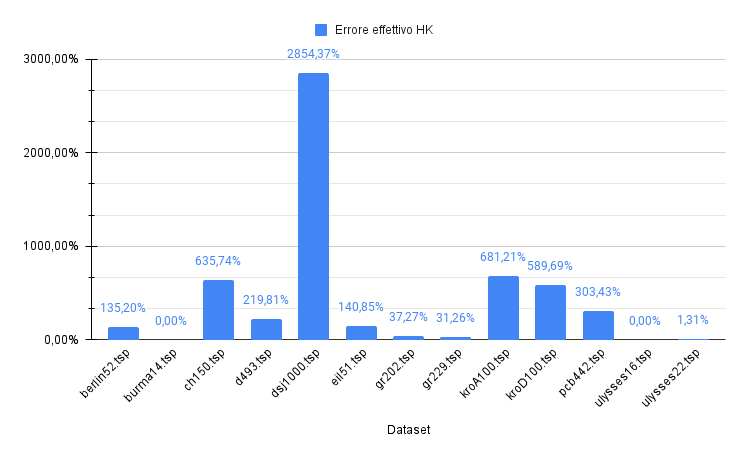
\includegraphics[width=0.85\textwidth]{res/images/errors/hk-effettivo.png}
	\caption{Errore effettivo dei risultati ottenuti con Held-Karp.}
	\label{fig:errors-hk-effettivo}
\end{figure}

\begin{figure}[H]
	\centering
	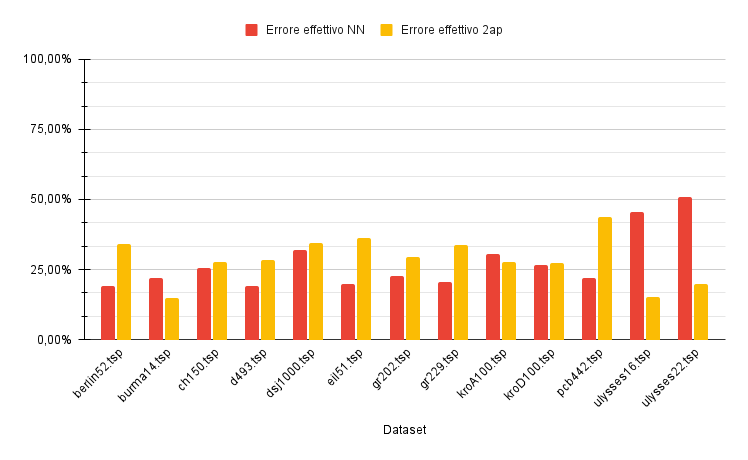
\includegraphics[width=0.85\textwidth]{res/images/errors/approx-effettivo.png}
	\caption{Errore effettivo dei risultati ottenuti con gli algoritmi non esatti.}
	\label{fig:errors-approx-effettivo}
\end{figure}

\begin{figure}[H]
	\centering
	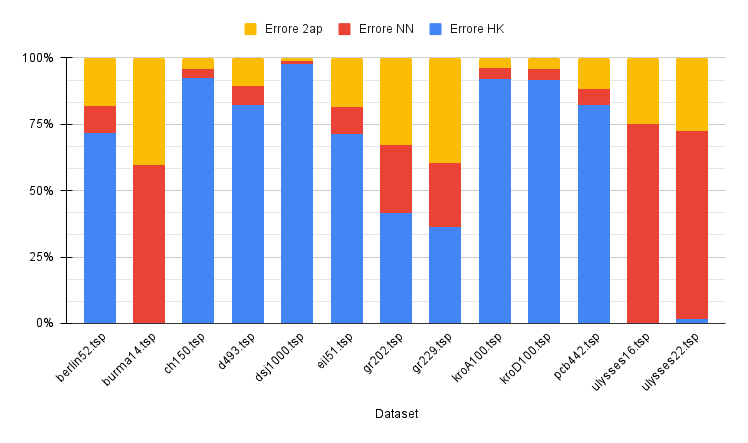
\includegraphics[width=0.85\textwidth]{res/images/errors/all.png}
	\caption{Errori in proporzione per i tre algoritmi.}
	\label{fig:errors-all}
\end{figure}

\begin{figure}[H]
	\centering
	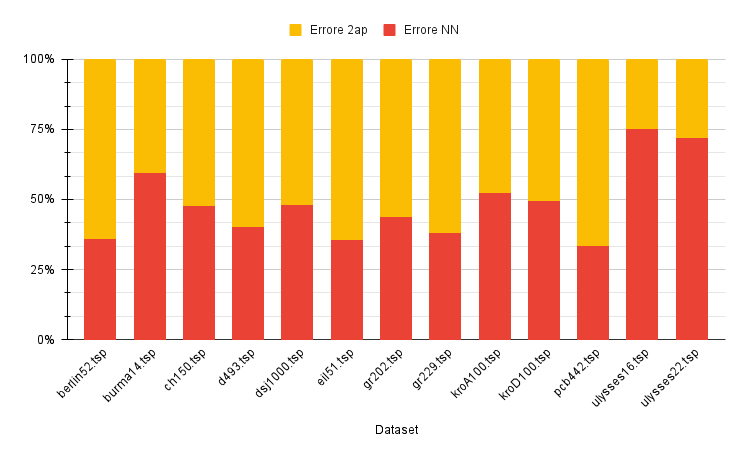
\includegraphics[width=0.85\textwidth]{res/images/errors/approx.png}
	\caption{Errori in proporzione per gli algoritmi non esatti.}
	\label{fig:errors-approx}
\end{figure}

Come si può evincere da questi grafici (fig. \ref{fig:errors-hk-effettivo}, \ref{fig:errors-approx-effettivo}, \ref{fig:errors-all}, \ref{fig:errors-approx}), l'algoritmo nearest neighbor sembra essere, \textit{in media}, più efficiente; ciò non è vero, però, per grafi più piccoli come \textit{burma14}, \textit{ulysses16} e \textit{ulysses22}, in cui l'algoritmo di 2-approssimazione si avvicina decisamente meglio alla soluzione ottima. 
Oltre alla complessità computazionale diversa, una possibile ipotesi che abbiamo avanzato nel corso dell'analisi di questi risultati potrebbe ricondursi alla natura \textit{greedy} dell'algoritmo nearest neighbor, che procede con la scelta ottima per ogni vertice incontrato. Pertanto, la potenzialità di questo algoritmo si riflette meglio con grafi di maggior dimensione proprio perché il numero di scelte da effettuare è maggiore e quindi il possibile tasso di errore si riduce in proporzione. Chiaramente questa ipotesi è puramente un'osservazione basata su nostre congetture che sarebbe interessante approfondire.


\begin{figure}[H]
	\centering
	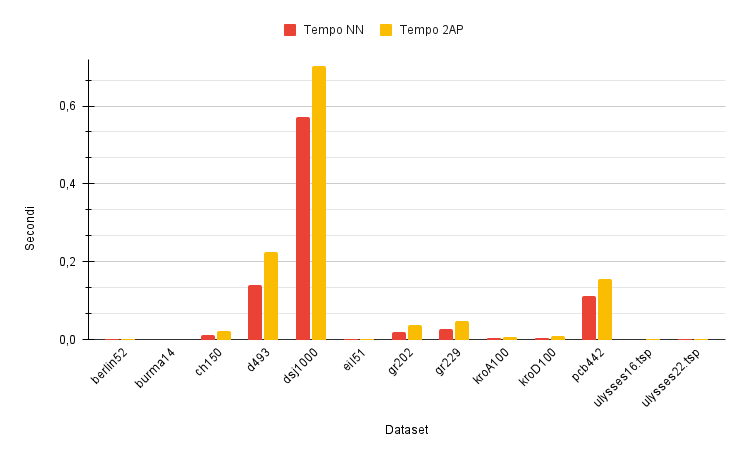
\includegraphics[width=1\textwidth]{res/images/time/time-nn-2ap.png}
	\caption{Tempi effettivi ottenuti con Nearest Neighbor e 2-approssimazione.}
	\label{fig:time-nn-2ap}
\end{figure}

Per quanto riguarda le tempistiche degli algoritmi di approssimazione, si può notare dal grafico \ref{fig:time-nn-2ap} che i tempi di esecuzione dei due algoritmi, anche ripetuti più e più volte, denotano un minore tempo di computazione effettivo per l'algoritmo di Nearest Neighbor, specialmente nei grafi più grandi. 
Analogamente, anche nei grafi di minore dimensione (fig. \ref{fig:time-detail-nn-2ap}) è possibile notare che questo algoritmo è quello che ci impiega meno tempo a livello computazionale, confermandosi quindi il più veloce dei tre. 

\begin{figure}[H]
	\centering
	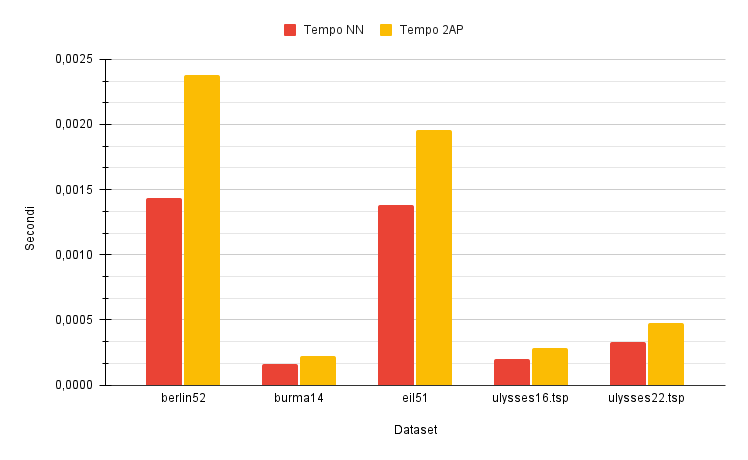
\includegraphics[width=1\textwidth]{res/images/time/time-detail-nn-2ap.png}
	\caption{Dettaglio dei tempi effettivi ottenuti con Nearest Neighbor e 2-approssimazione nei dataset più piccoli.}
	\label{fig:time-detail-nn-2ap}
\end{figure}

Per quanto concerne le tempistiche di Held and Karp, solo due dataset hanno computato il risultato entro tre minuti, mentre uno di questi, \textit{ulysses22}, ci è andato vicino con un errore del 1,31\% (fig. \ref{fig:errors-hk-effettivo}). Altri dataset, come \textit{burma14} e \textit{ulysses16}, hanno completato la computazione e hanno ottenuto in un tempo relativamente basso i risultati, rispettivamente di circa 0.35 e 1.96 secondi.